% 20230707
% Giovanni Ramirez
% ramirez@ecfm.usac.edu.gt

%
% Esta es una plantilla y contiene lo mínimo que debe llevar el protocolo de
% año de prácticas.  La portada es una propuesta y se puede ajustar según se
% desee.
%
% Esta plantilla se puede usar tanto en un compilador de LaTeX en su
% computadora o en algún compilador en línea como overleaf.com
%

\documentclass[titlepage,11pt]{article}

%%% PAQUETES
% esto es para hacer las cosas en español y para usar el punto como separador
% decimal
\usepackage[spanish,es-nodecimaldot]{babel}%
% esto es por la codificación con la que se escribe, revisar la codificación
% de su sistema pues podría estar en utf16 o en iso-latin-1 o iso 8859-1
\usepackage[utf8]{inputenc}%
% esto es para agregar gráficas y figuras
\usepackage{graphicx}%
% esto es por algunos símbolos como la ñ o las vocales tildadas
\usepackage{latexsym}%
% esto es para tener acceso a varios símbolos matemáticos
\usepackage{amsfonts, amsmath}%
% esto es para facilitar la escritura de algunos símbolos en física
\usepackage{physics}
\usepackage{float}
% esto es para poder usar el sistema internacional de unidades
\usepackage[amssymb]{SIunits}%
% esto es para que la página sea tamaño carta
\usepackage[letterpaper, bottom=25mm, top=25mm]{geometry}
% esto es para los colores, la opción table es para poner colores en las
% celdas
\usepackage[table]{xcolor}
% esto es para las tablas largas
\usepackage{longtable}
% esto es para poder escribir en varios renglones en la tabla
\usepackage{array}


% esto es útil para los hipervínculos y metadata
\usepackage[bookmarksnumbered, breaklinks={true},%
pdfauthor={Alejandro Barillas (alejandroecfm@gmail.com)},%
pdftitle={Redes neuronales de aprendizaje automático para la Inferencia de modelos físicos},%
pdfsubject={F\'isica Computacional},%
pdfkeywords={Physical Systems \& Artificial neural networks \& Machine learning}]{hyperref}


\begin{document}
% % % % % % % % % % % % % % % % % % % % % % % % % % % % % % % % % % %
% aquí se define la página de la portada, las distancias y tamaños son
% relativos al tamaño de la fuente que se define al inicio en documentclass
\begin{titlepage}
  % esto es para que no ponga número a la página
  \pagestyle{empty}
  % esto agrega el título a los bookmarks
  \pdfbookmark[0]{Title}{title}
  \begin{center}
    % esto es para los logos
    \begin{minipage}{\textwidth}
      \begin{minipage}[c]{0.45\textwidth}
        \centering 
\includegraphics[width=.8\textwidth]{usacAzul}
      \end{minipage}%
      \hfill
      \begin{minipage}[c]{0.45\textwidth}
        \vspace{-1em}
\includegraphics[width=.85\textwidth]{ecfmAzul}
      \end{minipage}
    \end{minipage}

    % esto pone los nombres de las instituciones
    \vspace{2em}
    \begin{minipage}[t]{.95\textwidth}
      \centering\large
      \textsc{Universidad de San Carlos de Guatemala\\
        Escuela de Ciencias Físicas y Matemáticas}
    \end{minipage}

    % esto pone la línea horizontal
    \vspace{1em}\noindent\rule{\textwidth}{1px}\vfill
    % esto pone el título
    \begin{minipage}[t]{.95\textwidth}
      \centering\Huge
      \textsc{Redes Neuronales de Aprendizaje Automático para la Inferencia de Modelos Físicos}
    \end{minipage}

    % esto pone los datos 
    \vfill
    \begin{minipage}[t]{.75\textwidth}
      \centering
      Anteproyecto de Año de Prácticas elaborado por\\%
      \textbf{Cesar Alejandro Barillas Segura}\\
      presentada ante el Departamento de Física
    \end{minipage}

    % esto pone más datos
    \vfill
    \begin{minipage}[t]{.95\textwidth}
      \centering
      Supervisado por \\%
      Dr. Giovanni Ramírez García (ECFM-USAC)
    \end{minipage}

    \vfill\noindent\rule{\textwidth}{1px}
    \begin{minipage}[t]{.95\textwidth}
      \centering
      Guatemala, Marzo de 2024
    \end{minipage}
  \end{center}
\end{titlepage}
% % % % % % % % % % % % % % % % % % % % % % % % % % % % % % % % % % %


% esto hace que el resumen no tenga número de página y que la introducción
% empiece con el número de página 1
\pagestyle{empty}
\setcounter{page}{0}

% % % % % % % % % % % % % % % % % % % % % % % % % % % % % % % % % % %
% en esta página se hace un resumen del trabajo, se recomienda que no exceda
% las 500 palabras.
%

% esto es para terminar la página del resumen y pasar a la nueva página con el
% número uno
\newpage
\pagestyle{plain}


% % % % % % % % % % % % % % % % % % % % % % % % % % % % % % % % % % %
% en esta sección se describe la institución donde se realizarán las
% prácticas, como es la USAC, ECFM e IFM no hace falta cambiar.
%
\section{Descripción general de la Institución}
\label{sec:institucion}
La Universidad de San Carlos de Guatemala (USAC) es la institución de
educación superior estatal, autónoma, con cultura democrática, con enfoque
multi e intercultural, vinculada y comprometida con el desarrollo científico,
social, humanista y ambiental, con una gestión actualizada, dinámica, efectiva
y con recursos óptimamente utilizados para alcanzar sus fines y objetivos. Es
la universidad más antigua de Guatemala, habiendo sido fundada el 31 de enero
de 1676. El campus central se encuentra ubicado en el Departamento de
Guatemala, Ciudad Universitaria 11 Avenida, Zona 12. Su lema es \emph{Id y
  enseñad a todos}.

La Escuela de Ciencias Físicas y Matemáticas (ECFM) es una escuela no
facultativa formada en el año 2009 en el evento CONVERGENCIA. Actualmente, la
escuela cuenta con la carrera de Licenciatura en Física Aplicada y
Licenciatura en Matemática Aplicada. La escuela cuenta también con un
Instituto dedicado a la investigación de las ciencias físicas y matemáticas
(IFIM) el cual ha presentado diversas investigaciones y publicado una variedad
de artículos relacionados con la divulgación del conocimiento de las ciencias.

El IFIM es la unidad de la ECFM que promueve y realiza estudios avanzados en
áreas científicas fundamentales y aplicadas de las ciencias físicas y
matemáticas.  Las áreas y líneas de investigación del Instituto son
\begin{enumerate}
\item Física de altas energías, cosmología y astrofísica: Física de
  partículas, Astrofísica de rayos gamma.
\item Ciencias no lineales y sistemas complejos: Materia condensada, Modelos
  numéricos del clima, Modelos matemáticos en ciencias de la salud.
\item Geofísica: Geodesia aplicada a la tectónica.  
\item Física experimental: Detección de partículas e instrumentación
  electrónica, Redes de sensores.  
\item Física de radiaciones: Control de calidad en radioterapia.  
\end{enumerate}

Además, el Instituto realiza actividades de difusión y divulgación, Seminarios
científicos, Conferencias de divulgación científica y también Talleres y
cursos cortos.


% % % % % % % % % % % % % % % % % % % % % % % % % % % % % % % % % % %
% en esta sección se describe el grupo de investigación donde se realizarán
% las prácticas, como es el Grupo de investigación en Física de la Materia
% condensada no hace falta cambiar nada.
%
\section{Descripción del grupo de trabajo}
\label{sec:grupo}
La Física de Materia Condensada es un área muy amplia e interesante. Mediante
el estudio de las propiedades fundamentales de la materia se pueden observar
fenómenos interesantes que permiten el desarrollo de nuevas tecnologías. En
años recientes la relación entre éstos fenómenos a nivel subatómico y las
propiedades generales de los materiales ha permitido el desarrollo de
materiales con nuevas propiedades o materiales de diseño.

Por otro lado, uno de los desarrollos más excitantes de la Física en los
últimos años es la convergencia entre la Física de la Materia Condensada y las
áreas de Información Cuántica y Computación Cuántica, lo que ha permitido un
avance acelerado en ambos campos llevando de la mano a la teoría y al
experimento. El principal motivo de esta convergencia es el estudio de los
sistemas cuánticos de muchos cuerpos donde es indispensable entender el
entrelazamiento cuántico que resulta ser el recurso principal para la teoría
de información cuántica.

El Grupo de investigación se enfoca en las áreas de la física de la materia
condensada, incluyendo varios grupos de estudio aplicados a mecánica
estadística, mecánica cuántica, óptica, nanociencia, información cuántica,
computación cuántica, etc.


% % % % % % % % % % % % % % % % % % % % % % % % % % % % % % % % % % %
% en esta sección se describe el proyecto y en subsecciones se van colocando
% los temas que se considere necesario agregar para que una persona que lea el
% anteproyecto pueda hacerse a la idea de lo que se va a trabajar.
%
\section{Introducción}
\label{sec:introduccion}
En este proyecto se aprenderá a programar, entrenar y estudiar las características internas de una Red Neuronal dedicada a la identificación de modelos físicos. Para este caso en particular estudiaremos la caída libre de partículas. Para la descripción de este movimiento usaremos la teoría de MRUV que se detalla en la sección \ref{subsec:mru}. Los conocimientos matemáticos  necesarios para la construcción de la red neuronal son cálculo y álgebra lineal. Algunos de estos conceptos se mencionan en la sección \ref{subsec:mat}. La parte técnica y descriptiva de las redes neuronales se menciona en la sección \ref{subsec:redneuronal}, en esta, se explica su arquitectura, cómo funciona, y algunas funciones que ayudan a optimizar la capacidad de cómputo de una red neuronal. Una vez programada, se tomarán datos experimentales, dejando caer una partícula. Se tomar\'an videos de las trayectorias y posteriormente se analizar\'an los tiempos y se entrenará la red con dicha información. Este entrenamiento es posible gracias al aprendizaje automático. De esto se da una idea en la sección \ref{subsec:ML}. Toda esta red será programada con TensorFlow, una tecnología desarrollada por Google para el desarrollo de redes neuronales; esto se menciona en \ref{subsec:ts}.

\subsection{Movimiento rectilíneo uniformemente variado}
\label{subsec:mru}

	Para el caso de la caída libre de una partícula con velocidad inicial $v_0$, durante un tiempo de caída $t_f$, la partícula habrá recorrido una distancia.
	
	$$\Delta y=v_0 t_f+\frac{1}{2}a t_f^2,$$

	La aceleración durante la caída libre es el valor de la gravedad. En este caso se dejará caer desde el reposo, lo que implicará que la velocidad inicial será cero. En este problema se toma el segundo término como positivo, ya que s\'olo estamos interesados en el cambio de posición de un punto $A$ a otro $B$ expresado como $\Delta y$, y el tiempo de caída. Como la aceleración está a favor del movimiento (la partícula acelera), la aceleración se toma como positiva.

\subsection{Herramientas Matemáticas}
\label{subsec:mat}

	\subsubsection{Suma Ponderada}
		Una neurona artificial toma entradas representadas como $(x_1, x_2, \ldots, x_n)$ y pesos representados como $(w_1, w_2, \ldots, w_n)$. La suma ponderada se calcula multiplicando cada entrada por su peso correspondiente y sumando los resultados.
		$$z = w_1 \cdot x_1 + w_2 \cdot x_2 + \ldots + w_n \cdot x_n + b .$$
		Donde $b$ es el sesgo, en otras palabras es un valor constante.\\
		
		La suma ponderada ajusta las entradas según su importancia relativa, determinada por los pesos. Estos pesos se adaptan durante el entrenamiento de la red neuronal {\cite{triola_2018_estadstica}}.
		
	\subsubsection{Regresión Lineal}
	
		Dada una colección de datos, la línea de regresión es la recta que mejor se ajusta a los datos. Esto bajo el criterio de mínimos cuadrados. La ecuación de regresión lineal es:
		
		$$\hat{y}=b_0+b_1 x.$$
		
		Esto sirve para saber qu\'e tan buenas son las predicciones hechas por el modelo {\cite{triola_2018_estadstica}}.
	
	
	\subsubsection{Derivadas Parciales}
	
		Las derivadas parciales proporcionan información crucial sobre cómo una función cambia con respecto a cada una de sus variables independientes. Esto puede servir para medir la tasa de cambio de la función en una dirección específica y encontrar los puntos críticos de una función. Para la función de varias variables $z=f(x_1,x_2,\ldots,x_n)$ respecto de una de sus variables se define como
		
		$${\partial z\over\partial a}=\lim\limits_{\Delta a\rightarrow0}{f(x_1,x_2,\ldots,a+\Delta a,\ldots,x_n)-f(x_1,x_2,\ldots,x_n)\over\Delta a},$$
		
		\noindent donde $a$ es cualquiera de las variables de la función. Esto determina la razón de cambio de una función respecto de la variable deseada {\cite{zill_1985_clculo}}.
	
	\subsubsection{Regla de la Cadena}
	
		Si $z=f(u_1,u_2,\ldots,u_n)$ y cada una de las variables $u_i$ son funciones de $x_1,x_2,\ldots,x_k$ entonces tenemos que \cite{zill_1985_clculo}
		
		$${\partial z\over\partial x_i}={\partial z\over\partial u_1}{\partial u_1\over\partial x_i}+{\partial z\over\partial u_2}{\partial u_2\over\partial x_i}+\cdots+{\partial z\over\partial u_n}{\partial u_n\over\partial x_i}.$$ 
		
		Donde $i$ puede tomar cualquier valor entero de 1 hasta $k$.
	
	\subsubsection{Divergencia}
		
		La divergencia en redes neuronales se utiliza para medir la disparidad entre dos distribuciones de probabilidad. En el contexto del aprendizaje automático, especialmente en técnicas de optimización, la divergencia se emplea para cuantificar qué tan lejos está una distribución aproximada de la verdadera distribución de los datos. Esto es se aplica en tareas como el entrenamiento de modelos generativos, donde se busca ajustar la distribución de salida del modelo lo más cercano posible a la distribución real de los datos, permitiendo una generación más precisa de nuevas muestras.\\
		
		La divergencia de un campo arbitrario $\vec{F}= P\hat{i}+Q\hat{j}+R\hat{k}$ es la función escalar dada por
		
		$$div \vec{F}=\nabla\cdot\vec{F}={\partial P\over\partial x}+{\partial Q\over\partial y}+{\partial R\over\partial z}.$$
		
		En el contexto de Redes Neuronales, la divergencia se utiliza en la función de pérdida durante el entrenamiento de redes neuronales para guiar la optimización de los pesos \cite{zill_1985_clculo}.


\subsection{Red Neuronal}
\label{subsec:redneuronal}

	\subsubsection{Neurona}
		Una red neuronal es un conjunto interconectado de nodos llamados neuronas artificiales. Estas neuronas están organizadas en capas y se comunican entre sí mediante conexiones ponderadas. Cada neurona procesa información y la transmite a otras neuronas a través de estas conexiones.
		
		Cada neurona toma la información de entrada, hace una suma ponderada, y transmite esta información a la siguiente neurona, o en su defecto como salida \cite{antonio_2023_introduccin}\cite{ibm_qu}\cite{santana_2018_1}\cite{santana_2018_2}\cite{santana_2018_3}\cite{santana_2018_3_5}.
	\subsubsection{Capas}
	
		Hay diferentes tipos de capas neuronales.
		\begin{itemize}
			\item{\bf Capa de entrada:} Recibe los valores de entrada de la red neuronal.
			\item {\bf Capas ocultas:} Procesan la información de manera intermedia.
			\item{\bf Capa de salida:} Dan los datos de salida de la red neuronal.
		\end{itemize}
		
		Cada neurona artificial se conecta a otras y tiene un peso y un umbral asociados. Si la salida de una neurona está por encima del valor de umbral especificado, se activa y envía datos a la siguiente capa de la red. De lo contrario, no se pasan datos a la siguiente capa \cite{antonio_2023_introduccin}\cite{ibm_qu}\cite{santana_2018_1}\cite{santana_2018_2}\cite{santana_2018_3}\cite{santana_2018_3_5}.
	
	\subsubsection{Función de Activación}
	
		La función determina la salida de una neurona a partir de sus entradas. Estas funciones se aplican a la suma ponderada de las entradas y los pesos de una neurona. Su función principal es permitir la incorporación de modelado de datos no lineales en la red y facilitar el proceso de aprendizaje \cite{wikipediacontributors_2018_activation}.\\
		
		Algunas de las funciones más comunes para un valor de x, donde  la variable $x$ representa el valor de la suma ponderada de las entradas y los pesos en una neurona, son:
		
		\begin{enumerate}
			\item {\bf Función Sigmoide:} Lleva los valores entre 0 y 1. Se utiliza especialmente para modelos en los que se necesita predecir probabilidades, como en la clasificación binaria. Su ecuación es:
			$$f(x)={1\over1+e^{-x}}$$
			
			\begin{figure}[H]
				\centering
				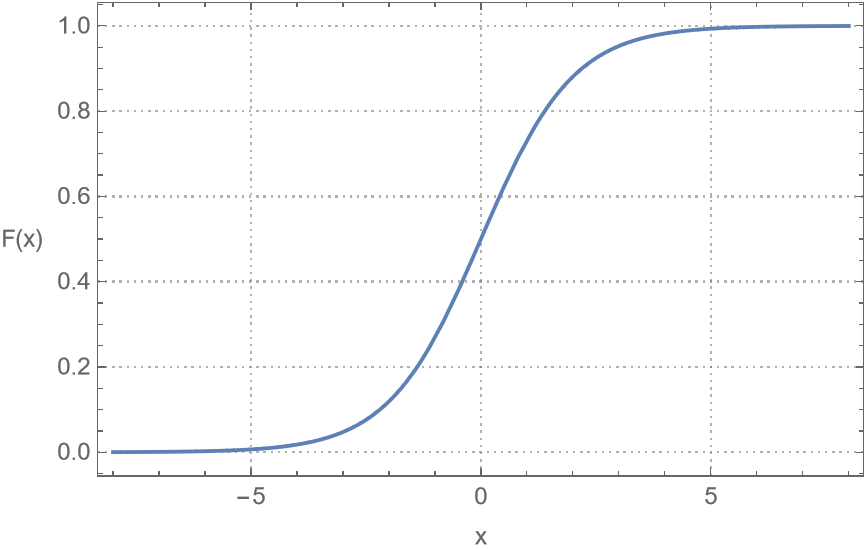
\includegraphics[width=0.4\linewidth]{sigmoide}
				\caption{Gráfica de la función sigmoide. Fuente: Elaboración propia.}
				\label{fig:sigmoide}
			\end{figure}
			
			
			\item {\bf Función Tangente Hiperbólica (tanh):} Su rango es de -1 a 1. Es similar a la función sigmoide, pero centrada en el origen. Se utiliza en redes neuronales para modelar relaciones no lineales. Su ecuación es:
			$$f(x)={e^{x}-e^{-x}\over e^{x}+e^{-x}}$$
			
			\begin{figure}[H]
				\centering
				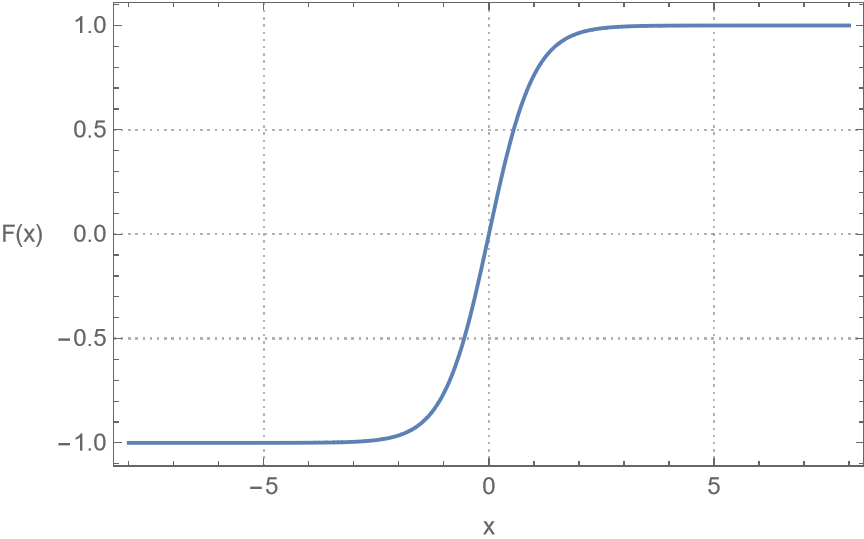
\includegraphics[width=0.4\linewidth]{tanh}
				\caption{Gráfica de la función Tangente Hiperbólica. Fuente: Elaboración propia.}
				\label{fig:tanh}
			\end{figure}
			
			\item {\bf Función Rectificadora Lineal (ReLU):} Es una función no lineal que devuelve 0 para valores negativos y el valor original para valores positivos. Su ecuación es:
			$$f(x)=\max(0,x)$$
			
			\begin{figure}[H]
				\centering
				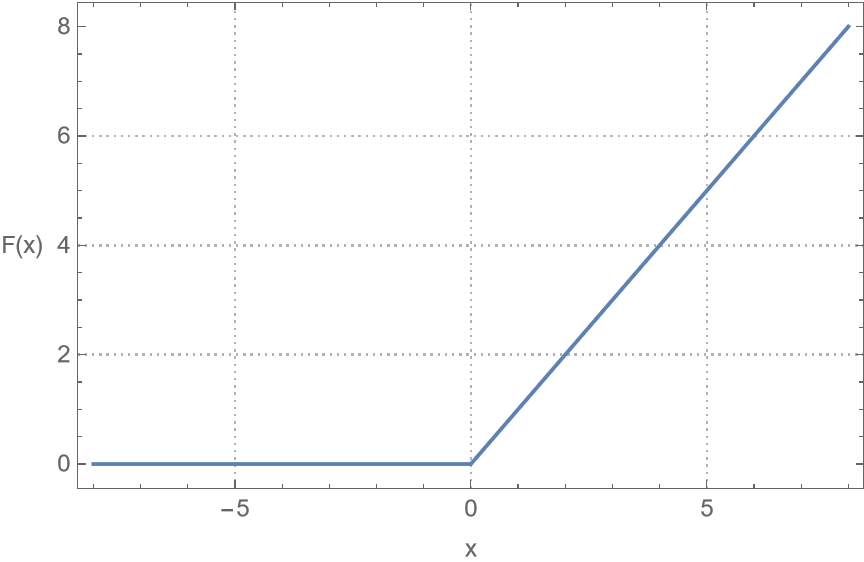
\includegraphics[width=0.4\linewidth]{relu}
				\caption{Gráfica de la función ReLU. Fuente: Elaboración propia.}
				\label{fig:relu}
			\end{figure}
			

		\end{enumerate}
	
	\subsubsection{Función de Coste}
	
		La función de coste en redes neuronales es crucial para determinar el error entre el valor estimado y el valor real durante el proceso de entrenamiento. Su objetivo principal es optimizar los parámetros de la red neuronal para que las predicciones se acerquen lo más posible a los valores reales. Algunas de las m\'as utilizadas son: \cite{antonio_2023_introduccin}\cite{ibm_qu}\cite{santana_2018_1}\cite{santana_2018_2}\cite{santana_2018_3}\cite{santana_2018_3_5}
		
		\begin{enumerate}
			\item {\bf Raíz Cuadrada Media (RMSE):} Calcula la raíz cuadrada media de los residuos, que son las diferencias entre los valores previstos $(V_p)$ y los valores reales $(V_r)$ 
			
			$$\text{RMSE} = \sqrt{\frac{1}{n} \sum_{i=1}^{n} (V_p - V_r)^2},$$
			
			$n$ es el número total de elementos en el conjunto de datos.
			
			\item {\bf Error Absoluto Medio (MAE):} Calcula la suma media de los valores absolutos de los errores. Es más fácil de interpretar que el RMSE, pero penaliza menos los valores grandes
			
			$$\text{MAE} = \frac{1}{n} \sum_{i=1}^{n} |x_i - x| ,$$
			
			donde $|x_i - x|$ representa los errores individuales y $n$ es el número total de elementos en el conjunto de datos.
			
			\item {\bf Error Absoluto Medio Escalado (MASE):} Similar al MAE pero escalado. También es más fácil de interpretar y simétrico.
			
			$$\text{MASE} = \frac{1}{n} \sum_{i=1}^{n} \left| \frac{q_i}{\text{MAE}} \right|,$$
			
			donde $n$ es el número de períodos de muestra de pronóstico, y $q_i$ representa los errores absolutos individuales.
		\end{enumerate}
		
		Además, existen optimizadores que trabajan con estas funciones de coste para ajustar los pesos de la red neuronal. Algunos ejemplos son:
		
		\begin{itemize}
			\item {\bf Descenso Estocástico del Gradiente (SGD):} Aproximación estocástica del gradiente descendente que busca minimizar una función objetivo.
			
			\item {\bf Adam:} Optimizador que adapta el ratio de aprendizaje en función de cómo están distribuidos los parámetros.
		\end{itemize}

\subsection{Aprendizaje Automático (Machine Learning)}
\label{subsec:ML}
	\subsubsection{Backpropagation}
		El backpropagation, también conocido como “propagación hacia atrás de errores”, es un algoritmo fundamental para el aprendizaje supervisado en redes neuronales artificiales. Su objetivo es ajustar los pesos de la red neuronal para minimizar el error entre las predicciones y los valores reales.
		

\subsection{TensorFlow}
\label{subsec:ts}
	TensorFlow es una plataforma de extremo a extremo enfocada en el aprendizaje automático. Es una biblioteca matemática simbólica que utiliza flujo de datos y programación diferenciable para realizar diversas tareas relacionadas con el entrenamiento e inferencia de redes neuronales profundas. TensorFlow es una plataforma de código abierto para el aprendizaje automático y el análisis de datos desarrollada por Google y liberada en 2015. Inicialmente, Google Brain, una división de investigación de inteligencia artificial de Google, desarrolló un sistema de aprendizaje automático llamado DistBelief. Para utilizar esta tecnología solo es necesaria la instalación de TensorFlow, se descarga e instala en un entorno de desarrollo, la descarga se puede hacer desde la p\'agina oficial \cite{TensorFlow}.  



% % % % % % % % % % % % % % % % % % % % % % % % % % % % % % % % % % %
% en esta sección hay que escribir los objetivos, para esto hay que tener en
% cuenta que los objetivos deben ser medibles, deben estar ordenados.
\section{Objetivos}
\label{sec:objetivos}
	


\subsection{General}
\label{sec:general}

\begin{itemize}
	\item Estudiar la teoría, ejercicios, experiencias e historia del aprendizaje automático para entender la estructura interna de las redes neuronales aplicadas a la elaboración de modelos matemáticos que describan el comportamiento de los datos de montajes experimentales de caída libre.. 
\end{itemize}

\subsection{Específicos}
\label{sec:especificos}

\begin{itemize}
	\item Estudiar el desarrollo histórico y aplicaciones del aprendizaje automático para la física.
	\item Entender el funcionamiento de las redes neuronales de aprendizaje automático.
	\item Construir redes neuronales básicas y entrenarlas.
	\item Entrenar una red neuronal con ejemplos de M.R.U.V.
\end{itemize}

% % % % % % % % % % % % % % % % % % % % % % % % % % % % % % % % % % %
% en esta sección hay que justificar el por qué es importante hacer este
% proyecto, también el por qué es importante que el/la estudiante lo haga.
\section{Justificación}
\label{sec:justificacion}
Las redes neuronales y los sistemas de aprendizaje automático están cada día más presentes en la sociedad. Estas herramientas, a pesar de ser el foco de discusiones éticas y morales, son de gran ayuda en diversas áreas: artísticas, de productividad, financieras y, en especial, científicas. Las herramientas de aprendizaje automático permiten la resolución de tareas complejas en segundos. Además, se ha demostrado que son muy buenas al momento de buscar patrones y crear “modelos” matemáticos, ya que en esencia su construcción es matemática.

Tomando esto en cuenta, la idea es familiarizarse con la estructura, entrenamiento y aspectos técnicos de las redes neuronales. Para posteriormente estudiar el modelo que utiliza la red neuronal para reproducir los resultados experimentales. Una vez terminado, se tendrá una herramienta que puede ayudar en la didáctica y divulgación de la ciencia y tecnología.\\

Se espera que esto siente las bases para el Ejercicio de Practica Supervisada EPS que pretende seguir con este estudio y generalizar algunos aspectos para diferentes marcos teóricos.

Se espera que esto siente las bases para el Ejercicio de Práctica Supervisada EPS que pretende seguir con este estudio y generalizar algunos aspectos para diferentes marcos teóricos.

La motivación personal es adquirir experiencia en áreas de interés personal, como lo son la física, tecnología y programación. Esto será una ayuda para desenvolverme en la industria o el mundo académico, según sea el caso. Esto sin desaprovechar la oportunidad de contribuir con la investigación nacional y el desarrollo tecnológico y científico de Guatemala. 




% % % % % % % % % % % % % % % % % % % % % % % % % % % % % % % % % % %
% en esta sección hay que explicar cómo se van a hacer las cosas que se
% quieren hacer, cómo se van a cumplir los objetivos que se plantearon,
% etc. También hay que hacer un listado de los recursos que se van a utilizar
% y hay que decir de dónde se van a sacar, por ejemplo: el libro tal lo voy a
% prestar en la biblioteca, el programa tal lo voy a escribir yo, el clúster
% para las simulaciones es el clúster Euclides de la ECFM
\section{Metodología}
\label{sec:metodologia}
El proyecto se basa en aprender; la teoría de las redes neuronales de aprendizaje automático, la programación y creación de redes neuronales, a estudiar la estructura de la red ya entrenada y probada.  Para esto se consultarán distintos libros, artículos y contenido audiovisual. Con esto se comienza con el desarrollo del proyecto con la ayuda de la bibliografía y resolución de dudas del asesor para poder crear las redes neuronales que servirán para aprender lo antes mencionado. Después se hace un boceto del documento final para que el asesor brinde sus sugerencias y correcciones. Por último, se tendrá listo el informe final de prácticas. 

% % % % % % % % % % % % % % % % % % % % % % % % % % % % % % % % % % %
% en esta sección hay que explicar en qué orden se van a hacer las cosas, qué
% tareas hay que completar antes de empezar a hacer las otras y así.  Se
% pueden colocar subtareas.
\section{Plan de trabajo}
\label{sec:plan}

Este anteproyecto se presenta el 2 de mayo de 2024.  Tras su aprobación sé
necesitarán 2 meses y dos semanas donde se trabajaran las tareas y se presentarán resultados
semanalmente

\begin{longtable}[h]{|l|c|c|c|c|c|c|c|c|c|c|}
  \hline & \multicolumn{4}{c|}{\textbf{Mes 1}} &
  \multicolumn{4}{c|}{\textbf{Mes 2}} & \multicolumn{2}{c|}{\textbf{Mes 3}}\\
  %
  \hline & \textbf{1}& \textbf{2}& \textbf{3}& \textbf{4} &
  \textbf{5}& \textbf{6}& \textbf{7}& \textbf{8} & \textbf{9}& \textbf{10} \\
  \hline
  %
  Tarea 1 & \multicolumn{1}{c}{\cellcolor{gray!50}}& & & & & & & & & \\ \hline
  Tarea 2 & & \multicolumn{2}{c}{\cellcolor{gray!50}} & & & & & & & \\ \hline
  Tarea 3 & & & & \multicolumn{2}{c}{\cellcolor{gray!50}} & & & & & \\ \hline
  Tarea 4 & & & & & & \multicolumn{2}{c}{\cellcolor{gray!50}} & & & \\ \hline
  Tarea 5 & & & & & & & & \multicolumn{2}{c}{\cellcolor{gray!50}}  & \\ \hline
  Tarea 6 & & & & & & & & & &\multicolumn{1}{c}{\cellcolor{gray!50}} \\ \hline
\end{longtable}

Las tareas están distribuidas así
\begin{description}
\item[Tarea 1:] Elaboración del estado del arte de el problema.
	\begin{description}
		\item[Subtarea 1:] Delimitar los tipos de movimiento.
	\end{description}
\item[Tarea 2:] Familiarizarse con el lenguaje de programación.
	\begin{description}
		\item[Subtarea 1:] Programar redes neuronales para entender el funcionamiento del lenguaje. 
		\item[Subtarea 2:] Estudiar la estructura de dichas redes.
	\end{description}
\item[Tarea 3:] Estructura de la red neuronal.
	\begin{description}
		\item[Subtarea 1:] Esquematizar la estructura para la red neuronal.
		\item[Subtarea 2:] Tomar los datos para el entrenamiento y limpiar datos.
	\end{description}
\item[Tarea 4:] Entrenamiento de la Red Neuronal.
\item[Tarea 5:] Estudio de la estructura de la red entrenada.
\item[Tarea 6:] Conclusiones y elaboración de informe final.
\end{description}


% % % % % % % % % % % % % % % % % % % % % % % % % % % % % % % % % % %
% en esta sección hay que comentar las referencias que se van a usar

\section{Bibliografía}
\label{sec:biografia}

\subsection*{Referencias comentadas}
\label{sec:referencias}

Todo lo pertinente a teoría física será tomado de Blatt \cite{Fisica}. La referencia estadística predeterminada será el libro de Mario \cite{triola_2018_estadstica}. La parte matemática es consultada en el libro de cálculo, será el de Zill \cite{zill_1985_clculo}. El canal de YouTube llamado DotCSV es una referencia audiovisual bastante completa en cuanto a redes neuronales se refiere \cite{santana_2018_1,santana_2018_2,santana_2018_3,santana_2018_3_5}. Para consultas técnicas rápidas y recomendaciones de la comunidad se usará la página de Wikipedia sobre "Función de activación" \cite{wikipediacontributors_2018_activation}. Las ayudas para entender el lenguaje serán tomadas de Amita y Martínez \cite{Amita}. 

Como documentación complementaria, usaremos el libro de \cite{Jesus} para la parte del lenguaje.


% esta versión usa Bibtex para generar las referencias que están en archivo
% adjunto con el nombre referencias.bib.  Hay varios estilos, los básicos son:
% abbrv, acm, alpha, apalike, ieeetr, plain, siam, unsrt
\bibliographystyle{ieeetr}% otras opciones {plain}
\bibliography{referencias}
\end{document}


%%% Local Variables:
%%% mode: latex
%%% TeX-master: t
%%% End:
